%%%%%%%%%%%%%%%%%%%%%%%%%%%%%%%%%%%%%%%%%
% Beamer Presentation
% LaTeX Template
% Version 1.0 (10/11/12)
%
% This template has been downloaded from:
% http://www.LaTeXTemplates.com
%
% License:
% CC BY-NC-SA 3.0 (http://creativecommons.org/licenses/by-nc-sa/3.0/)
%
%%%%%%%%%%%%%%%%%%%%%%%%%%%%%%%%%%%%%%%%%

%----------------------------------------------------------------------------------------
%	PACKAGES AND THEMES
%----------------------------------------------------------------------------------------

\documentclass{beamer}

\usepackage{ctex}

\usepackage{textpos}
%% 根据需要修改中文字体
\setCJKmainfont[ItalicFont={SimSun}]{SimSun}
% \setCJKsansfont{Microsoft YaHei}
\setCJKsansfont{SimHei}
\setCJKmonofont{FangSong_GB2312}

% \setCJKmonofont{SimSun}
% \xeCJKsetcharclass{"0}{"2E7F}{0}
% \xeCJKsetcharclass{"2E80}{"FFFF}{1}

% Require XeLaTeX
\RequirePackage{fontspec,xltxtra,xunicode}
% 根据需要修改英文字体
\setmainfont[Mapping=tex-text]{Times New Roman}
\setsansfont[Mapping=tex-text]{Arial}
\setmonofont{Consolas}
%
%% 设置公式字体
\usefonttheme[onlymath]{serif}

\setbeamertemplate{caption}[numbered]
\setbeamertemplate{bibliography item}[text]
\mode<presentation> {
	
	% The Beamer class comes with a number of default slide themes which change the colors and layouts of slides. Below this is a list of all the themes, uncomment each in turn to see what they look like.
	%
%\usecolortheme{beaver}
%	\usetheme{default}
%	\usetheme{AnnArbor}
%	\usetheme{Antibes}
%	\usetheme{Bergen}
%	\usetheme{Berkeley}
%	\usetheme{Berlin}
%	\usetheme{Boadilla}
%	\usetheme{CambridgeUS}
%	\usetheme{Copenhagen}
%	\usetheme{Darmstadt}
%	\usetheme{Dresden}
%	\usetheme{Frankfurt}
%	\usetheme{Goettingen}
%	\usetheme{Hannover}
%	\usetheme{Ilmenau}
%	\usetheme{JuanLesPins}
%	\usetheme{Luebeck}
	\usetheme{Madrid}
%	\usetheme{Malmoe}
	%\usetheme{Marburg}
%	\usetheme{Montpellier}
%	\usetheme{PaloAlto}
%	\usetheme{Pittsburgh}
	%\usetheme{Rochester}
%	\usetheme{Singapore}
%	\usetheme{Szeged}
	%\usetheme{Warsaw}
	
	% As well as themes, the Beamer class has a number of color themes
	% for any slide theme. Uncomment each of these in turn to see how it
	% changes the colors of your current slide theme.
	
%	\usecolortheme{albatross}
%	\usecolortheme{beaver}
%	\usecolortheme{beetle}
%	\usecolortheme{crane}
%	\usecolortheme{dolphin}
%	\usecolortheme{dove}
%	\usecolortheme{fly}
%	\usecolortheme{lily}
%	\usecolortheme{orchid}
%	\usecolortheme{rose}
%	\usecolortheme{seagull}
%	\usecolortheme{seahorse}
%	\usecolortheme{whale}
%	\usecolortheme{wolverine}
	
	%\setbeamertemplate{footline} % To remove the footer line in all slides uncomment this line
%	\setbeamertemplate{footline}[page number] % To replace the footer line in all slides with a simple slide count uncomment this line
	
	\setbeamertemplate{navigation symbols}{} % To remove the navigation symbols from the bottom of all slides uncomment this line
}
%\usepackage{bookman} % the used font
\usepackage{graphicx} % Allows including images
\usepackage{booktabs} % Allows the use of \toprule, \midrule and \bottomrule in tables
%\usepackage{pgf}  

\newcommand{\omegab}{{\vo{\omega}}}
\newcommand{\vo}[1]{\boldsymbol{#1}}


% 设置logo
%\pgfdeclareimage[width=3cm]{university-logo}{logo1.jpg} %[height=2cm, width=2cm]
%\logo{\pgfuseimage{university-logo}}


%----------------------------------------------------------------------------------------
%	TITLE PAGE
%----------------------------------------------------------------------------------------
\title[无人机姿态估计] %optional %可以只写一个简短题目,或者写其他信息
{具有低功耗微处理器的\\
	小型无人机非线性姿态估计}

%\subtitle{A short story}

\author[姓名] % (optional, for multiple authors)
{姓名 }
%\author[The author]{
\includegraphics[width=2cm]{logo1}\\The Author}

\institute[SCUT] % (optional)
{
%	\inst{1}%
	华南理工大学 \\
	xxxx重点实验室\\
	广东省xxxx中心	
	
}

\date[2022年11月]% (optional)
{2022年11月}


\logo{
\includegraphics[height=0.6cm]{logo1}}

%\logo{\pgfputat{\pgfxy(9.45,1.5)}{\pgfbox[center,base]{
\includegraphics[width=1.7cm]{logo1.jpg}}}} 

%\titlegraphic{%
%	\begin{picture}(0,0)
%		\put(305,-120){\makebox(0,0)[rt]{
\includegraphics[width=2cm]{logo1.jpg}}}
%\end{picture}}
%----------------------------------------------------------------------------------------
%	Highlight the title of the current section
%----------------------------------------------------------------------------------------
\AtBeginSection[]
{
	\begin{frame}
		\frametitle{目录}
		\tableofcontents[currentsection]
	\end{frame}
}



%----------------------------------------------------------------------------------------
%	All pages in the slides
%----------------------------------------------------------------------------------------
\begin{document}
	% no page #, no logo on title page

	% insert title page---------------------------
	\frame{\titlepage}
	
	%insert contents------------------------------
	\begin{frame}
		\frametitle{目录}
		\tableofcontents
	\end{frame}
%	\addtobeamertemplate{frametitle}{}{%
%	\begin{textblock*}{100mm}(0.75\textwidth,-0.75cm)
%		
\includegraphics[width=3cm]{logo1}
%	\end{textblock*}}
	\section{简介}
	
	\begin{frame}
		\frametitle{论文原文}
		
		{\Large Nonlinear Attitude Estimation for Small UAVs with Low Power Microprocessors}
		 
		\begin{itemize}
			\item Sunsoo Kim
			\item Vaishnav Tadiparthi
			\item Raktim Bhattacharya
		\end{itemize}
		Published in: 2020 American Control Conference (ACC)
	\end{frame}

	\begin{frame}
		\frametitle{研究背景}
		
		随着无人机往小型化发展,对计算高效的姿态估计算法的需求渐长。
		现阶段在无人机中应用最广泛的估计算法是EKF,有以下缺点:
		\begin{itemize}
			\item 卡尔曼增益需要两个步骤:传播与更新,需要较多的计算资源。
			\item 需要更多的内存。
			\item 假设的高斯不确定性模型不合理。
		\end{itemize}

	\end{frame}


	% insert a sample frame without animation--------------------------------
%	\begin{frame}
%		\frametitle{研究背景}
%		
%		随着无人机往小型化发展,对计算高效的姿态估计算法的需求渐长。
%		
%		\begin{itemize}
%			\item Text visible on slide 1
%			\item Text visible on slide 2
%			\item Text visible on slide 3 % pay attention to this line, you can omit the content by omit the '-'
%			\item Text visible on slide 4
%		\end{itemize}
%		
%	\end{frame}
	
	% insert a sample frame with animation 1 ----------------------------------
%	\begin{frame}
%		\frametitle{Sample frame title with animation}
%		This is a text in second frame. For the sake of showing an example.
%		
%		\begin{itemize}
%			\item<1-> Text visible on slide 1
%			\item<2-> Text visible on slide 2
%			\item<3> Text visible on slide 3 % pay attention to this line, you can omit the content by omit the '-'
%			\item<4-> Text visible on slide 4
%		\end{itemize}
%		
%	\end{frame}
%	
%	
%	% insert a sample frame with animation 2 -----------------------------------
%	\begin{frame}
%		In this slide \pause
%		
%		the text will be partially visible \pause
%		
%		And finally everything will be there
%	\end{frame}
	
	
	
	\section{预备知识}
	
	\begin{frame}
		\frametitle{传感器建模}
		
		陀螺仪模型:
		\begin{multline}\label{Gyro_M}
			\begin{pmatrix} \dot{\vo{\Phi}} \\ \dot{\vo{b}} \end{pmatrix}
			= \begin{bmatrix} \vo{0} & -\vo{T}(\vo{\Phi})\\ \vo{0}_{3\times3} & \vo{0}_{3\times3}\end{bmatrix}\begin{pmatrix}\vo{\Phi}\\\vo{b}\end{pmatrix} + 
			\begin{bmatrix}-\vo{T}(\vo{\Phi}) & \vo{0}_{3\times3} \\ \vo{0}_{3\times3} & I\end{bmatrix}\begin{pmatrix}\vo{n}_\omegab\\\vo{n_b}\end{pmatrix} + 
			\begin{pmatrix}\vo{T}(\vo{\Phi})\\\vo{0}_{3\times3}\end{pmatrix}\omegab_m,
		\end{multline}
		其中 
		\begin{align} \vo{\Phi}:= \begin{pmatrix} \phi \\ \theta \\ \psi \end{pmatrix}, \quad \nonumber
			\vo{T}(\phi,\theta,\psi) :=
			\begin{bmatrix}
				1 & \tan\theta \sin\phi & \tan\theta \cos\phi \\
				0 & \cos\phi            & -\sin\phi \\
				0 & \sin\phi \sec\theta & \cos\phi \sec\theta
			\end{bmatrix}, \nonumber
		\end{align}
	\begin{align}
	 ^B \omegab = \omegab_m - \vo{b} - \vo{n}_\omegab, \quad
		 \dot{\vo{b}} = \vo{n_b}. \nonumber
	\end{align}\label{gyro_m}
	\end{frame}

	\begin{frame}
		\frametitle{传感器建模}
		设:
		\begin{align}
			\vo{x}(t) =
			\begin{bmatrix}
				\vo{\Phi}\\
				\vo{b}
			\end{bmatrix},\nonumber
		\end{align}
		则陀螺仪模型为
		\begin{align}
			\vo{\dot{x}} = \vo{f}(\vo{x},\vo{u},\vo{w},t). \label{eqn:nldyn}
		\end{align}
	    且噪声$\begin{pmatrix}\vo{n_w}\\\vo{n_b}\end{pmatrix}$的协方差矩阵为:
	    \begin{gather}
	    	\vo{Q} =
	    	\begin{bmatrix}
	    		\vo{N}_w & \vo{0}_{3\times3}\\
	    		\vo{0}_{3\times3} & \vo{N}_b
	    	\end{bmatrix}
	    	=
	    	\begin{bmatrix}
	    		n^2_w\vo{I}_{3\times3} & \vo{0}_{3\times3}\\
	    		\vo{0}_{3\times3} & n^2_b \vo{I}_{3\times3}
	    	\end{bmatrix}.\nonumber
	    \end{gather}
	\end{frame}	

	\begin{frame}
		\frametitle{传感器建模}
		
		加速度计模型:
		\begin{align}\label{Acc_model}
			{}^B \vo{a} = {\vo{R}^{B}_I}_{acc} (\vo{\Phi}) \hspace{0.1cm} {}^I\vo{g}
		\end{align}
		其中
		\begin{align}
			{}^B{\vo{a}} &= \vo{a}_m - \vo{n}_a \nonumber
		\end{align}
		\begin{align}
			\vo{R}^B_I =&
			\begin{bmatrix}\nonumber
				1 &0 &0\\ 0 &\cos(\phi)& \sin(\phi)\\ 0& -\sin(\phi)& \cos(\phi)
			\end{bmatrix} \times
			\begin{bmatrix}
				\cos(\theta)& 0& -\sin(\theta)\\ 0& 1& 0\\ \sin(\theta)& 0& \cos(\theta)
			\end{bmatrix}\\ \times
			&
			\begin{bmatrix}
				\cos(\psi)& \sin(\psi)& 0\\ -\sin(\psi)& \cos(\psi)& 0\\ 0& 0& 1
			\end{bmatrix}.\nonumber
		\end{align}
	\end{frame}

	\begin{frame}
		\frametitle{传感器建模}
		
		磁力计模型:
		\begin{align}
			{}^B \vo{m} = {\vo{R}^B_I}_{mag} (\vo{\Phi}) \hspace{0.1cm} {}^I \vo{h} \label{mag_model}.
		\end{align}
	其中
	\begin{align}
		^B{\vo{m}} &= \vo{m}_m - \vo{n}_m  \label{phi_dot} \nonumber
	\end{align}
	噪声$\begin{pmatrix}\vo{n_a}\\\vo{n_m}\end{pmatrix}$的协方差矩阵为
	\begin{gather}
		\vo{R} =
		\begin{bmatrix}
			\vo{N}_a & \vo{0}_{3\times3}\\
			\vo{0}_{3\times3} & \vo{N}_m
		\end{bmatrix}
		=
		\begin{bmatrix}
			n^2_a \vo{I}_{3\times3} & \vo{0}_{3\times3}\\
			\vo{0}_{3\times3} & n^2_m \vo{I}_{3\times3}
		\end{bmatrix}. \nonumber
	\end{gather}
	\end{frame}

	\begin{frame}
		\frametitle{$\mathcal{H}_2$ 最优估计}
		
		考虑线性系统
	\begin{subequations}\label{system_CT}
		\begin{align}
			\Dot{\vo{x}}(t) &=  \vo{A} \vo{x}(t) + \vo{B}_u \vo{u}(t) + \vo{B}_w \vo{w}(t),\\
			\vo{y}(t) &= \vo{C}_y \vo{x}(t) + \vo{D}_u \vo{u}(t)+ \vo{D}_w \vo{w}(t),\\
			\vo{z}(t) &= \vo{C}_z \vo{x}(t),
		\end{align}
	\end{subequations}
 其 $\mathcal{H}_2$ 状态观测器为:
		\begin{subequations} \label{estimation_CT}
			\begin{align}
				\Dot{\hat{\vo{x}}}(t) &= \vo{A} \hat{\vo{x}}(t) + \vo{B}_u \vo{u}(t) + \vo{L} (\vo{C}_y \hat{\vo{x}}(t) + \vo{D}_u \vo{u}(t) - \vo{y}(t)),\\
				\hat{\vo{z}}(t) &= \vo{C}_z \hat{\vo{x}}(t),
			\end{align}
		\end{subequations}
	其误差方程为:
	\begin{subequations} \label{estimator_Linear}
		\begin{align}
			\hat{\Dot{\vo{e}}}(t) &= (\vo{A}+\vo{L} \vo{C}_y) \hat{\vo{e}}(t) + (\vo{B}_w+\vo{L} \vo{D}_w)\vo{w}(t), \\
			\Tilde{\vo{z}}(t) &= \vo{C}_z \hat{\vo{e}}(t).
		\end{align}
	\end{subequations}
	\end{frame}


\begin{frame}
	\frametitle{$\mathcal{H}_2$ 最优估计}
	$\mathcal{H}_2$ 状态观测器的设计问题是: 给定系统 (\ref{estimator_Linear}) 和一个正定标量 $\gamma$,寻找一个 $\vo{L}$ 使得:
	\begin{align}\label{min1}
		\|\vo{G}_{\Tilde{z}w}(s)\|_{2} < \gamma
	\end{align}
其中系统传递函数$\vo{G}_{\Tilde{z}w}(s)$表达式为:
\begin{align}\label{errorTF}
	\vo{G}_{\Tilde{z} w}(s) = \vo{C}_z [s \vo{I} -( \vo{A} + \vo{L} \vo{C}_y)]^{-1} (\vo{B}_w + \vo{L} \vo{D}_w) .
\end{align}
\end{frame}

\begin{frame}
	\frametitle{$\mathcal{H}_2$ 最优估计}
	$\mathcal{H}_2$ 最优估计\textbf{定理 } \cite{duan2013lmis, apkarian2001continuous} :以下两种陈述等价:
	\begin{enumerate}
		\item $\mathcal{H}_2$ 状态观测器的解$\vo{L}$存在.
		\item $\exists \vo{W}$, 且存在对称矩阵 $\vo{Q}$、$\vo{X}$ 使得:
		       \begin{align}\label{CT_LMI}
			\begin{bmatrix}\nonumber
				\vo{XA}+\vo{W} \vo{C}_y +(\vo{XA}+\vo{W} \vo{C}_y)^T &  \vo{X} \vo{B}_w+\vo{W} \vo{D}_w\\
				\vo{*}      & -\vo{I}
			\end{bmatrix}
			< 0,\\
			\begin{bmatrix}\nonumber
				\vo{-Q}  &  \vo{C}_z\\
				\vo{*} & \vo{-X}
			\end{bmatrix}
			< 0,\\
			\textbf{trace}(\vo{Q}) < \gamma^2.
		\end{align}
	\end{enumerate}
此时$\mathcal{H}_2$最优观测器增益为$\vo{L} = \vo{X}^{-1} \vo{W}$,此增益保证当$t \rightarrow \infty $时,$ \vo{e}(t) = \vo{x}(t) - \hat{\vo{x}} \rightarrow 0 $。
并且$\hat{\vo{x}}(t)$是$\vo{x}(t)$的渐进观测。
\end{frame}
	\section{解决方法}
	\begin{frame}
		\frametitle{扩展 $\mathcal{H}_2$ 估计}
		\begin{figure}[h!]
			\centering
			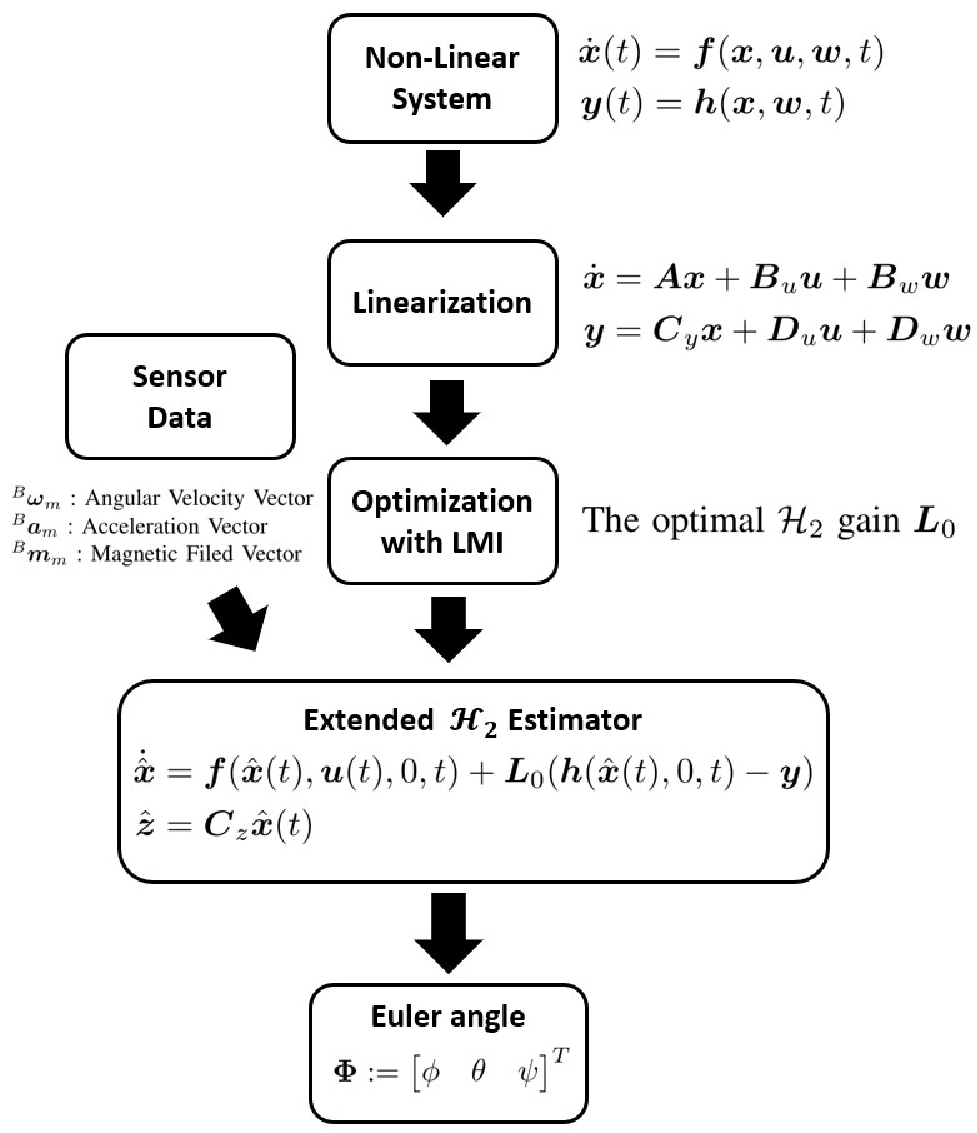
\includegraphics[trim={1cm 1cm 1cm 0.4cm},scale=0.41]{flow2.pdf}
			\caption{估计算法}
			\label{algorithm}
		\end{figure}
	\end{frame}
	
	
	\begin{frame}
		\frametitle{扩展 $\mathcal{H}_2$ 估计}
		回顾式 (\ref{eqn:nldyn}), 陀螺仪模型是一个非线性模型,重新表述为:
		\begin{align}\label{sys_eq}
			\Dot{\vo{x}} &= \vo{f}(\vo{x},\vo{u},\vo{w},t),
		\end{align}
其中 $\vo{u}(t) := \omegab_m(t)$ , $\vo{w}(t):=\begin{bmatrix}
	\vo{n}_\omegab(t)\\
	\vo{n}_b(t)
\end{bmatrix}$.
		
		
		另一方面,磁力计和加速度计的观测模型(\ref{Acc_model}, \ref{mag_model})可以写为:
		\begin{align} \label{eqn:measureEQ}
			\vo{y}(t) &= \vo{h}(\vo{x},\vo{w},t) = \vo{R}^B_I(\vo{\Phi})
			\begin{bmatrix}
				\vo{g} \\ \vo{h}
			\end{bmatrix}  + \vo{D}_w \vo{w}(t),
		\end{align}
		其中
		\vspace{-.3cm}
		\begin{gather*}
			\vo{R}^B_I(\vo{\Phi})
			=
			\begin{bmatrix}
				\vo{R}_{acc}(\vo{\Phi})& \vo{R}_{mag}(\vo{\Phi})
			\end{bmatrix},
			\vo{D_w} =
			\begin{bmatrix}
				\vo{I}_{3\times3} & \vo{0}_{3\times3}\\
				\vo{0}_{3\times3} & \vo{I}_{3\times3}
			\end{bmatrix}.
		\end{gather*}
	\end{frame}


\begin{frame}
	\frametitle{扩展 $\mathcal{H}_2$ 估计}
	状态方程在标称工作点 $(\vo{x}_0,\vo{u}_0, \vo{w}_0) = \vo{0}$ 处进行线性化,得
	\begin{align}
		\vo{f}&(\vo{x}(t), \vo{u}(t), \vo{w}(t), t) \approx \vo{f}(\vo{x}_0, \vo{u}_0,\vo{w}_0, t)\\ \nonumber
		&+\frac{\partial \vo{f} (\vo{x},\vo{u},t)}{\partial \vo{x}}\Bigg|_{\text{nominal}} \vo{x}(t)  +\frac{\partial \vo{f} (\vo{x},\vo{u},t)}{\partial \vo{u}}\Bigg|_{\text{nominal}} \vo{u}(t)\\ \nonumber
		&+ \frac{\partial \vo{f} (\vo{x},\vo{u},t)}{\partial \vo{w}}\Bigg|_{\text{nominal}} \vo{w}(t) + \textrm{H.O.T.}
	\end{align}
并将雅可比矩阵定义为:
\begin{align} \nonumber
	\vo{A}  := \frac{\partial \vo{f}(\vo{x},\vo{u},t)}{\partial \vo{x}}\Bigg|_{\text{nominal}},
	\vo{B}_u  := \frac{\partial \vo{f}(\vo{x},\vo{u},t)}{\partial \vo{u}}\Bigg|_{\text{nominal}},\\
	\vo{B}_w  := \frac{\partial \vo{f}(\vo{x},\vo{u},t)}{\partial \vo{w}}\Bigg|_{\text{nominal}}.
\end{align}
\end{frame}

\begin{frame}
	\frametitle{扩展 $\mathcal{H}_2$ 估计}
	同样观测方程\eqref{eqn:measureEQ} 可以线性化为:
	\begin{align}
		\vo{h}(\vo{x}(t), \vo{w}(t), t) \approx \nonumber\\
		\vo{h}(\vo{x_0}, \vo{w_0}, t) &+\frac{\partial \vo{h} (\vo{x},t)}{\partial \vo{x}}\Bigg|_{\text{nominal}} \vo{x}(t)\nonumber\\
		&+ \frac{\partial \vo{h} (\vo{x},t)}{\partial \vo{v}}\Bigg|_{\text{nominal}} \vo{w}(t) + \textrm{H.O.T.}
	\end{align}
	雅可比矩阵定义为:
	\begin{align}
		\vo{C}_y  := \frac{\partial \vo{h} (\vo{x},t)}{\partial \vo{x}}\Bigg|_{\text{nominal}},
		\vo{D}_w  := \frac{\partial \vo{h} (\vo{x},t)}{\partial \vo{w}}\Bigg|_{\text{nominal}}.\nonumber
	\end{align}
\end{frame}

\begin{frame}
	\frametitle{扩展 $\mathcal{H}_2$ 估计}
	线性化后的状态方程和观测方程为:
	 \begin{align}
		\Dot{\vo{x}}(t) &= \vo{f}(\vo{x}(t),\vo{u}(t),\vo{w}(t),t)\\
		&\approx \vo{f}(\vo{x_0},\vo{u_0}, t) + \vo{A} \vo{x}(t) + \vo{B_u} \vo{u}(t) + \vo{B_w} \vo{w}(t) .\nonumber
	\end{align}
 \begin{align}
	\vo{y}(t) &= \vo{h}(\vo{x}(t),\vo{w}(t),t)\\
	&\approx \vo{h}(\vo{x_0},\vo{w_0}, t) + \vo{C}_y \vo{x}(t) + \vo{D}_w(t) \vo{w}(t).\nonumber
\end{align}
可以等价于如下系统的估计问题:
\begin{subequations}\label{Lin_systems}
	\begin{align}
		\Dot{\vo{x}} &=  \vo{A}  \vo{x} + \vo{B}_u  \vo{u} + \vo{B}_w  \vo{w},\\
		\vo{y} &= \vo{C}_y  \vo{x} + \vo{D}_u  \vo{u}+ \vo{D}_w  \vo{w}.
	\end{align}
\end{subequations}
最优的$\mathcal{H}_2$增益$\vo{L}_0$然后可以通过求解(\ref{CT_LMI})中的优化问题来确定,其中下标$0$表示确定 关于标称工作点。
\end{frame}

\begin{frame}
	\frametitle{扩展 $\mathcal{H}_2$ 估计}
	一旦确定了增益 $\vo{L}_0$,它就用于为非线性系统实现 $\mathcal{H}_2$ 滤波器。 文章提出了一个新的实现,称为扩展 $\mathcal{H}_2$ 滤波器,其中滤波器状态使用非线性动力学传播。 在传统的 $\mathcal{H}_2$ 滤波器中,误差传播使用线性系统发生。 扩展的 $\mathcal{H}_2$ 滤波器的滤波器动态和输出方程由下式给出
	\begin{subequations}\label{estimator}
		\begin{align}
			\Dot{\Hat{\vo{x}}} &= \vo{f}(\hat{\vo{x}}(t),\vo{u}(t),0,t) +  \vo{L}_0(\vo{h}(\Hat{\vo{x}}(t),0,t) - \vo{y}),\\
			%    &= \vo{A}(\hat{\vo{x}}) \hat{\vo{x}}(t) + \vo{B}(\hat{\vo{x}})\vo{u}(t) +  \vo{L}_E(\vo{h}(\Hat{\vo{x}}) - \vo{y})\\
			\hat{\vo{z}} &= \vo{C}_z \hat{\vo{x}}(t).
		\end{align}
	\end{subequations}
\end{frame}
	
	\section{结果}
	
	% insert a sample frame with a figure -----------------------------------
	\begin{frame}
		\frametitle{仿真设置}
		所提出的扩展$\mathcal{H}_2$滤波器应用于姿态估计问题,其性能与基于扩展卡尔曼滤波器的姿态估计相比。 如图 \ref{sim_chart} 所示,比较是在基于 MATLAB 的仿真环境中的估计精度和计算时间方面进行的。
		\begin{figure}[h!]
			\centering
			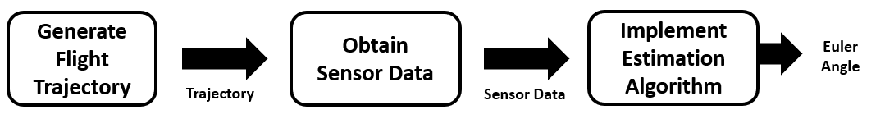
\includegraphics[width=\textwidth]{flow.pdf}
			\caption{仿真流程}
			\label{sim_chart}
		\end{figure}
	\end{frame}
	
	
		\begin{frame}
		\frametitle{仿真设置}
		噪声水平、偏差等传感器特性由 MPU 9250 的传感器数据表 \cite{MPU} 设置。在 MATLAB 仿真中,IMU 数据由 \texttt{imuSensor} 函数 \cite{MAT} 生成。 数据如图 \ref{IMU_Low} 所示。 文章使用两个飞行场景来验证所提出的扩展 $\mathcal{H}_2$ 估计算法。
		\begin{figure}[h!]
			\centering
			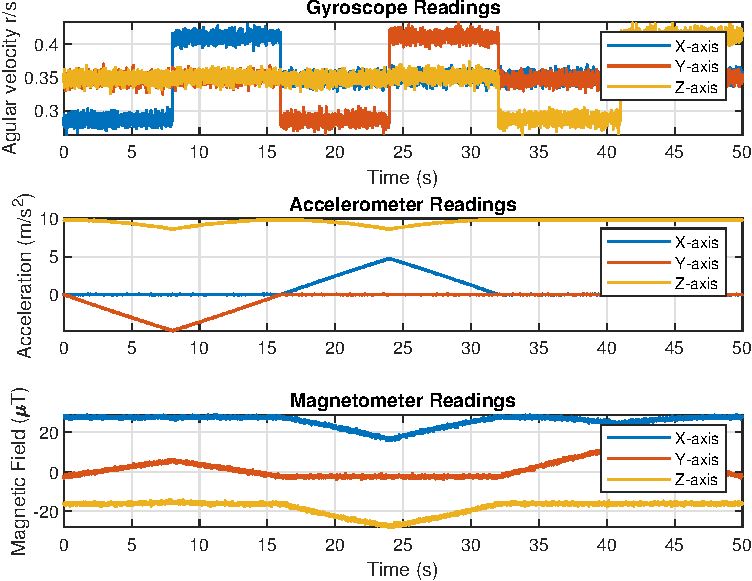
\includegraphics[width=0.6\textwidth]{Lowangle2.pdf}
			\caption{从Matlab函数 \textsl{imuSensor} 生成的 MPU- 9250 数据}
			\label{IMU_Low}
		\end{figure}
	\end{frame}

	\begin{frame}
	\frametitle{仿真设置}
	\textbf{案例 I:慢速和小角度运动},考虑围绕三个轴的角运动 $< 30^{\circ}$。 涵盖通常情况下四旋翼无人机的前/后和左/右巡航飞行。 仿真运行持续时间为 50 秒,角速度为 $\pi/50$ rad/s。 模拟的真实状态轨迹如图 \ref{Tra_Low} 所示。
	\begin{figure}[h!]
		\centering
		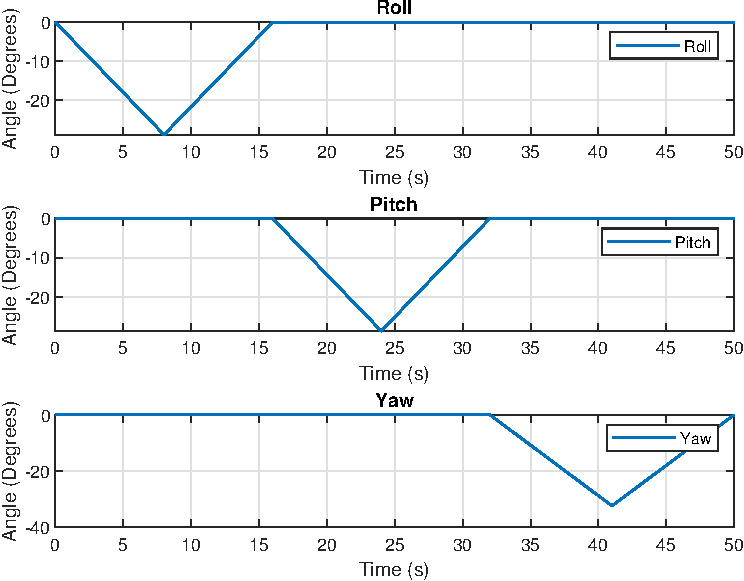
\includegraphics[width=0.47\textwidth]{Lowangle1.pdf}
		\caption{案例 I的欧拉角的真实轨迹}
		\label{Tra_Low}
	\end{figure}
\end{frame}


	\begin{frame}
	\frametitle{仿真设置}
	\textbf{案例 II:快速和大角度运动},考虑同时围绕三个轴的角度变化 $> 30^{\circ}$。 表示在飞行或激进机动过程中存在风扰动的情况下快速移动或运动的场景。 仿真运行持续时间为 10 秒,角速度为 $\pi/3$ rad/s。 模拟的真实状态轨迹如图 \ref{Tra_high} 所示。
	\begin{figure}[h!]
		\centering
		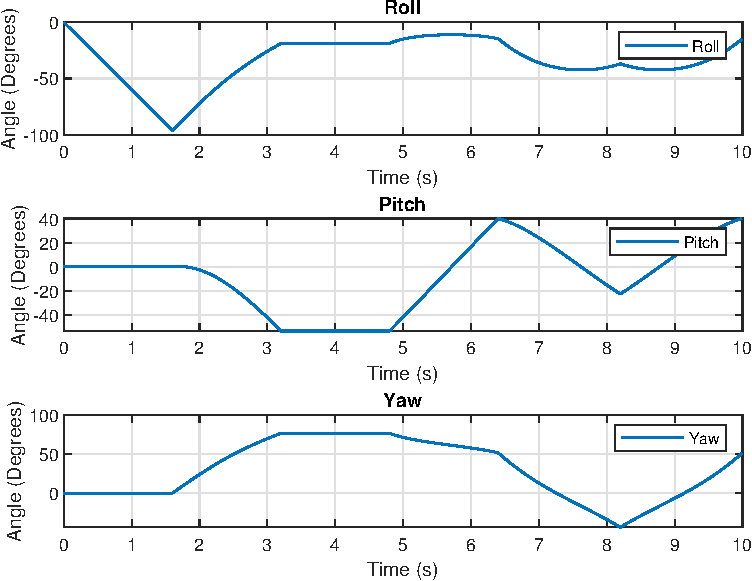
\includegraphics[width=0.47\textwidth]{highangle1.pdf}
		\caption{案例 II 的欧拉角的真实轨迹}
		\label{Tra_high}
	\end{figure}
\end{frame}

	\begin{frame}
		\frametitle{仿真结果}
		\textbf{案例 I:} 
		\begin{figure}[h]
			\centering
			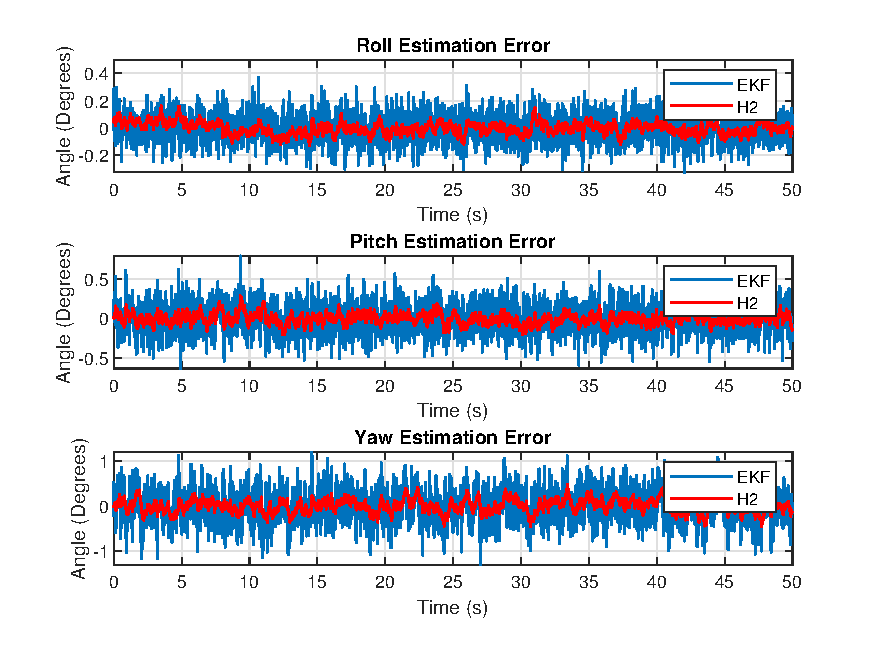
\includegraphics[width=0.7\textwidth]{EH2_lowangle.pdf}
			\caption{案例 I中,扩展 $\mathcal{H}_2$ 滤波器与 EKF 比较}
			\label{comp_low}
		\end{figure}
	\end{frame}

\begin{frame}
	\frametitle{仿真结果}
	\textbf{案例 I:} 
	\begin{table}[h]
		\caption{案例 I的RMS 误差} \label{RMS_low}
		\vspace{-0.3cm}
		\begin{center}
			\renewcommand{\arraystretch}{1.5}
			\begin{tabular}{|c||c|c|c|}
				\hline
				Algorithm & Roll angle (${}^\circ$) & Pitch angle (${}^\circ$) & Yaw angle (${}^\circ$)\\
				\hline \hline
				Extended $\mathcal{H}_2$ & 0.0331 & 0.0538 & 0.1107\\
				\hline
				EKF & 0.0533 & 0.0988 & 0.2298\\
				\hline
			\end{tabular}
		\end{center}
	\end{table}
\begin{table}[h]
	\caption{案例I的min-max误差}\label{min-max_low}
	\vspace{-0.2cm}
	\begin{center}
		\renewcommand{\arraystretch}{1.5}
		\begin{tabular}{|c||c|c|c|}
			\hline
			Algorithm & Roll angle (${}^\circ$) & Pitch angle (${}^\circ$) & Yaw angle (${}^\circ$)\\
			\hline \hline
			Extended $\mathcal{H}_2$ &  [-0.152 0.125] & [-0.284 0.240] & [-0.423 0.402]\\
			\hline
			EKF & [-0.257 0.249] & [-0.523 0.444]& [-1.087 0.937]\\
			\hline
		\end{tabular}
	\end{center}
\end{table}

\end{frame}

\begin{frame}
	\frametitle{仿真结果}
\textbf{案例 II:} 
\begin{figure}[h]
	\centering
	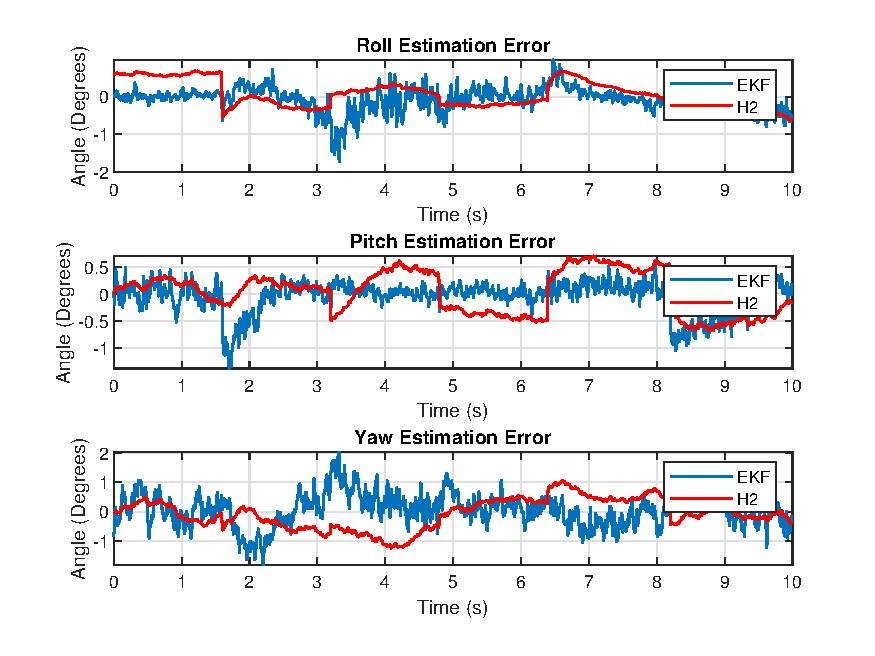
\includegraphics[width=0.7\textwidth]{EH2_highangle.pdf}
	\caption{案例 II 中,扩展 $\mathcal{H}_2$ 滤波器与 EKF 比较}
	\label{comp_high}
\end{figure}
\end{frame}


\begin{frame}
	\frametitle{仿真结果}
	\textbf{案例 II:} 
\begin{table}[h]
	\caption{案例 II的RMS 误差} \label{RMS_high}
	\vspace{-0.3cm}
	\begin{center}
		\renewcommand{\arraystretch}{1.5}
		\begin{tabular}{|c||c|c|c|}
			\hline
			Algorithm & Roll angle (${}^\circ$) & Pitch angle (${}^\circ$) & Yaw angle (${}^\circ$)\\
			\hline \hline
			Extended $\mathcal{H}_2$ & 0.3045 & 0.3260 & 0.3121\\
			\hline
			EKF & 0.3073 & 0.2656 & 0.5275\\
			\hline
		\end{tabular}
	\end{center}
\end{table}
\begin{table}[h!]
	\caption{案例II的min-max误差} \label{min-max_high}
	\vspace{-0.3cm}
	\begin{center}
		\renewcommand{\arraystretch}{1.5}
		\begin{tabular}{|c||c|c|c|}
			\hline
			Algorithm & Roll angle (${}^\circ$) & Pitch angle (${}^\circ$) & Yaw angle (${}^\circ$)\\
			\hline \hline
			Extended $\mathcal{H}_2$ &  [-0.592    0.730] & [-0.897    0.602] & [-0.857 0.664]\\
			\hline
			EKF & [-2.212   1.404] & [-1.84000.692] & [-2.227    3.097]\\
			\hline
		\end{tabular}
	\end{center}
\end{table}
\end{frame}

	
	\section{结论}
	% insert a sample frame with citation --------------------------------
	\begin{frame}
		\frametitle{结论}
		本文提出了一种新的非线性估计框架,基于 $\mathcal{H}_2$ 最优状态估计,用于低功耗微处理器中的姿态估计。且:
		\begin{itemize}
			\item 与广泛使用的 EKF 算法的性能相当。
			\item 所提出的框架的主要优势是计算效率高。
			\item 在计算不确定性方面的稳健性更佳。
		\end{itemize}
提出的姿态估计算法对于具有低功率微处理器的小型无人机非常有吸引力。 
	\end{frame}
	
	
	% insert a reference frame before the 'thank you' frame ----------------------
	\begin{frame}
		\frametitle{References}
		
%		\begin{thebibliography}{99} % Beamer does not support BibTeX so references must be inserted manually as below
%			\bibitem{team2015common}
%			Team, C.: Common vulnerability scoring system v3. 0: Specification document.
%			First. org  (2015)
%			
%			\bibitem{eiram2013cvssv2}
%			Eiram, C., Martin, B.: The cvssv2 shortcomings, faults, and failures
%			formulation. In: Technical report, Forum of Incident Response and Security
%			Teams (FIRST) (2013)
%			
%		\end{thebibliography}
\bibliographystyle{elsarticle-num}
\bibliography{H2filtering}
	\end{frame}
	
	
	% Insert a thank your frame ------------------------------------------------
	\begin{frame}
		\Huge{\centerline{谢谢!}}
	\end{frame}
	
\end{document}